
\chapter{MONTAJE}
Se le ofrece a continuación de estas líneas, un diagrama de bloques en el que se pueden apreciar los distintos componentes que se han utilizado y cómo se conectan entre sí.
\begin{figure}[h!]
\centering
\begin{tikzpicture}[node distance=4cm]
  \node (Shield) [Shield,draw] at(0,0) {Shield};
  \node (CNY70) [CNY70, draw] at (6,0){CNY70};
  \node (Sharp) [Sharp, draw] at (6,2) {Sharp};
  \node (HC-06) [HC-06, draw] at (-6,0){HC-06};
  \node (Ultrasonido) [Ultrasonido, draw] at(-6,2) {Ultrasonidos};
  \node (LED RGB) [RGB, draw] at (-6,-2){LED RGB};
  \node (Motores) [Motores, draw] at (6,-2) {Motores};
  \node (Bateria) [Bateria, draw] at (0,2) {Batería};
  \node (ArduinoLeonardo) [ArduinoLeonardo, draw] at (0,-4) {Arduino Leonardo};

  \draw[arrow] (CNY70)--(Shield);
  \draw[arrow] (Sharp)--(Shield);
  \draw[arrow] (HC-06)--(Shield);
  \draw[arrow] (LED RGB)--(Shield);
  \draw[arrow] (Motores)--(Shield);
  \draw[arrow] (Ultrasonido)--(Shield);
  \draw[arrow] (Bateria)--(Shield);
  \draw[darrow] (Shield)--(ArduinoLeonardo);

\end{tikzpicture}
\caption{Elementos del robot}
\end{figure}

Antes de mostrar el resultado final, nos gustaría mostrar el proceso seguido hasta llegar a la versión final del robot. Se muestra en primer lugar el diseño de las piezas 3D, con la mejora del uso de soportes en formas de árbol, para que no hubiese ningún problema durante la impresión.

\begin{figure}[h!]
  \centering
  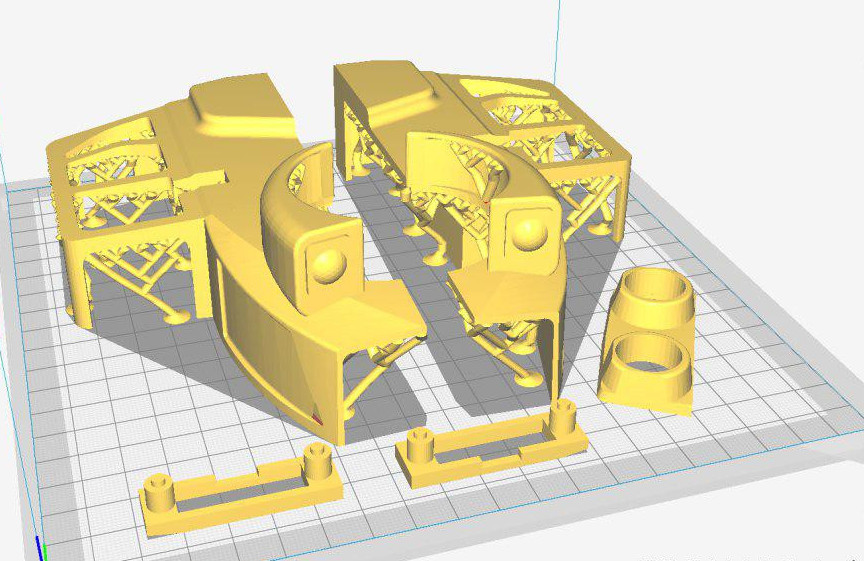
\includegraphics[scale=0.40]{img/DCE2.jpg}
  \caption{Diseño de las piezas 3D}
  \label{B}
\end{figure}

\

\

Se observa a continuación el resultado de las piezas impresas para el ultrasonidos y los sharp.

\begin{figure}[h!]
  \centering
  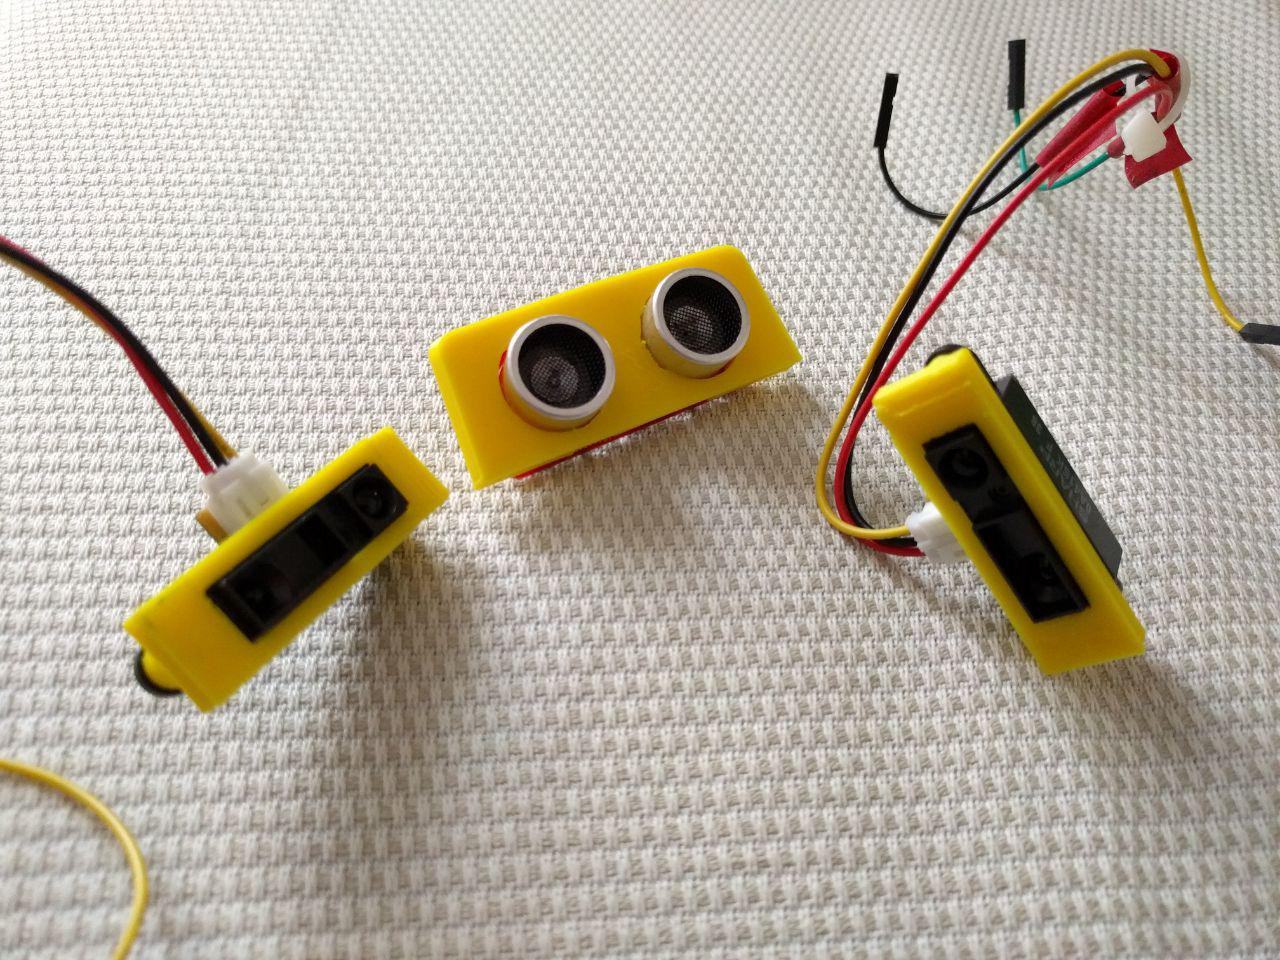
\includegraphics[scale=0.30]{img/DCE1.jpg}
  \caption{Piezas del Ultrasonidos y los Sharp}
  \label{A}
\end{figure}

Tras unir todas las piezas, éste es el aspecto del robot:

\begin{figure}[h!]
  \centering
  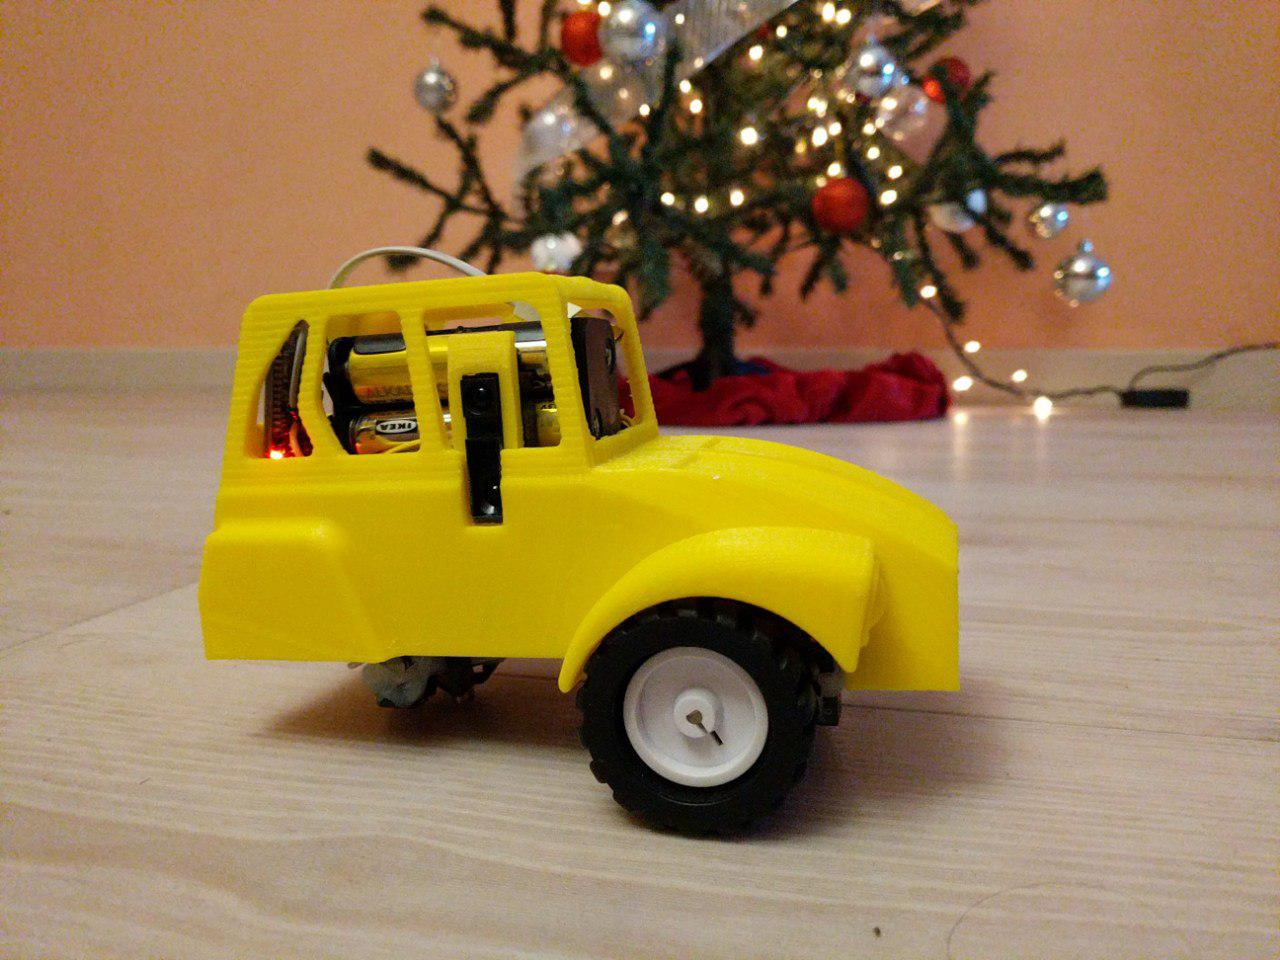
\includegraphics[scale=0.30]{img/Caprito.jpg}
  \caption{Imagen del robot con su chásis}
  \label{A}
\end{figure}

Se muestra además, una pequeña galería del robot en general:

\begin{figure}[h!]
\centering
\begin{tabular}{ccc}
  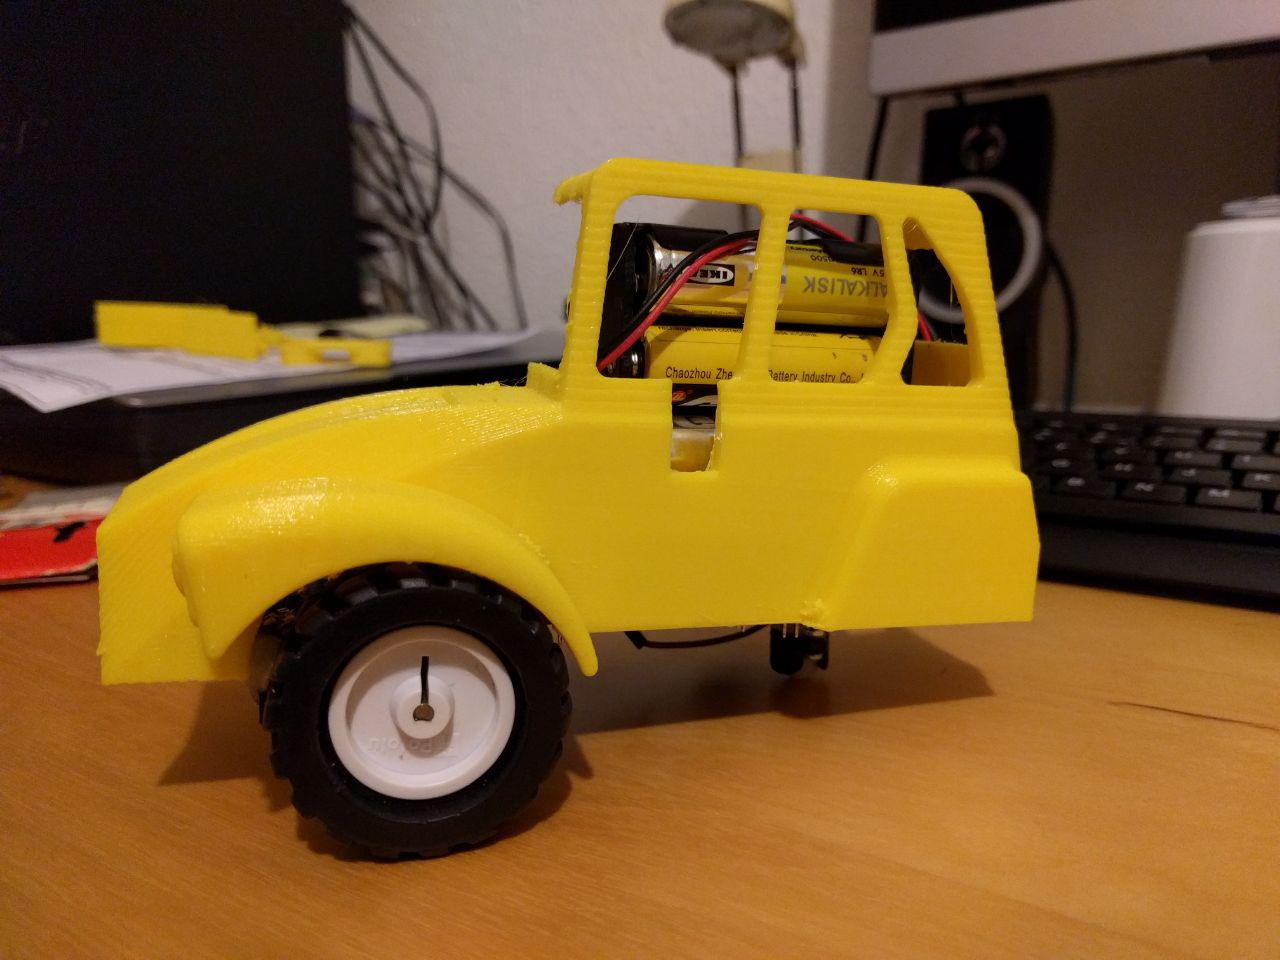
\includegraphics[width=150px, height=150px]{img/Caprito2.jpg}
&
  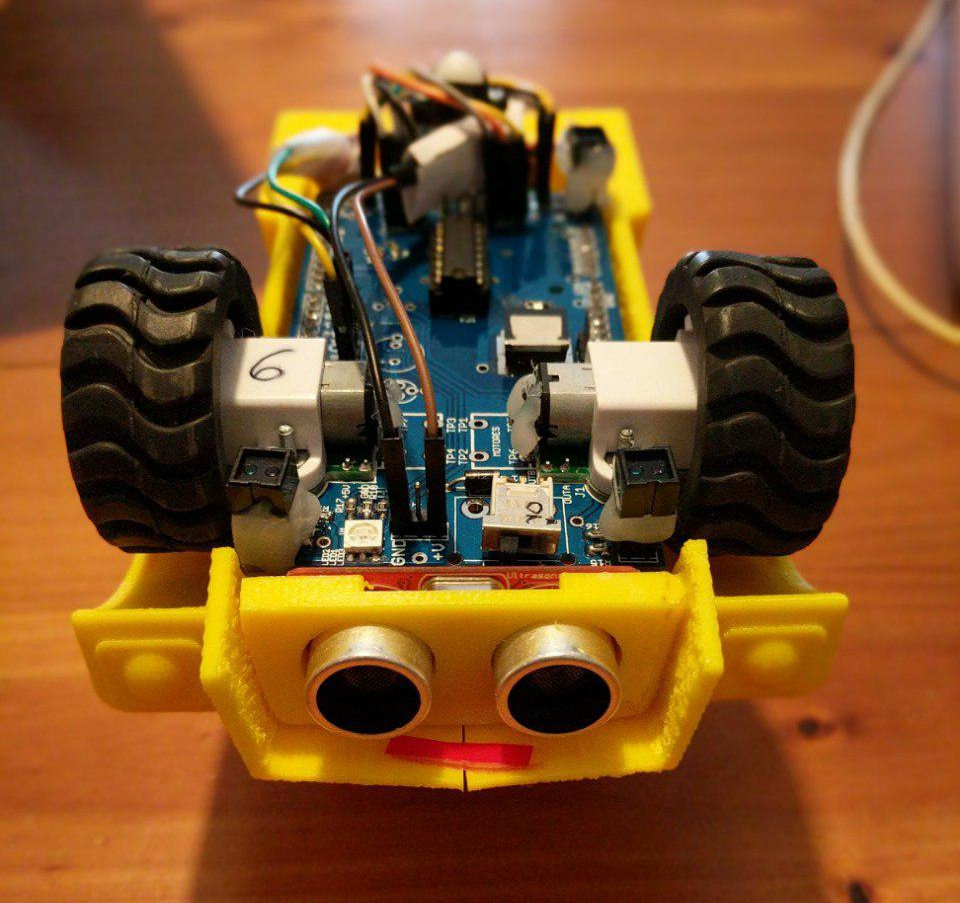
\includegraphics[width=150px, height=150px]{img/Caprito6.jpg}
  &
  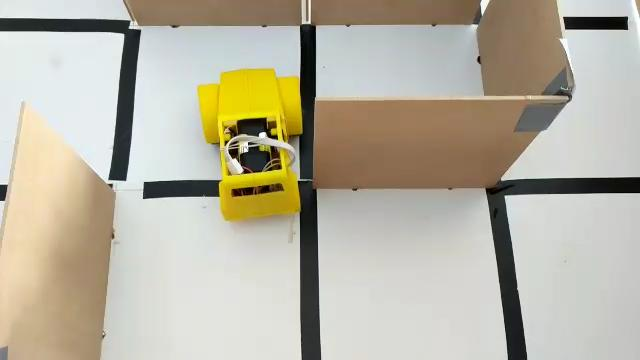
\includegraphics[width=150px, height=150px]{img/Caprito4.jpg}\\
  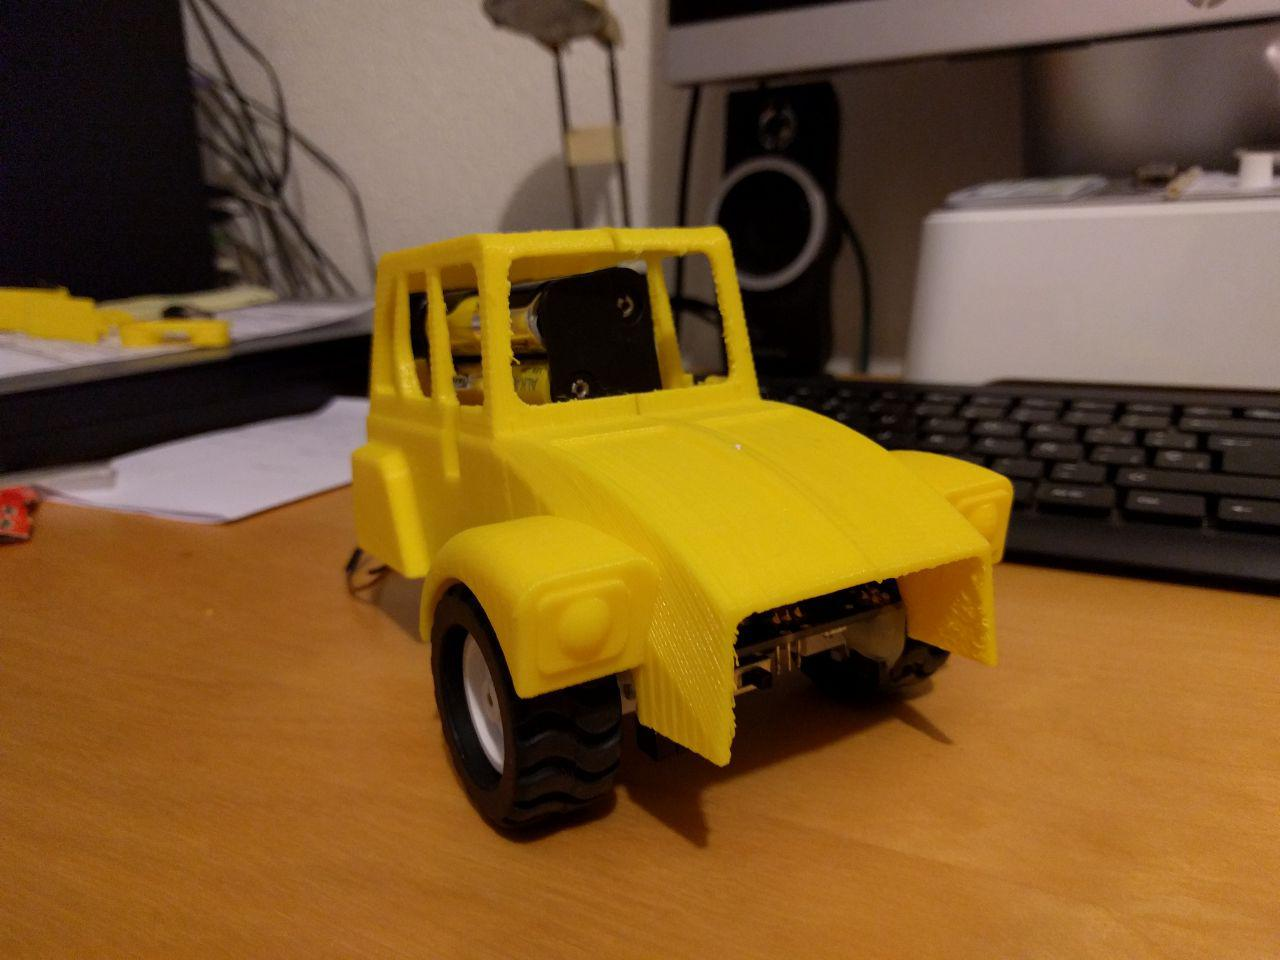
\includegraphics[width=150px, height=150px]{img/Caprito5.jpg}
  &
  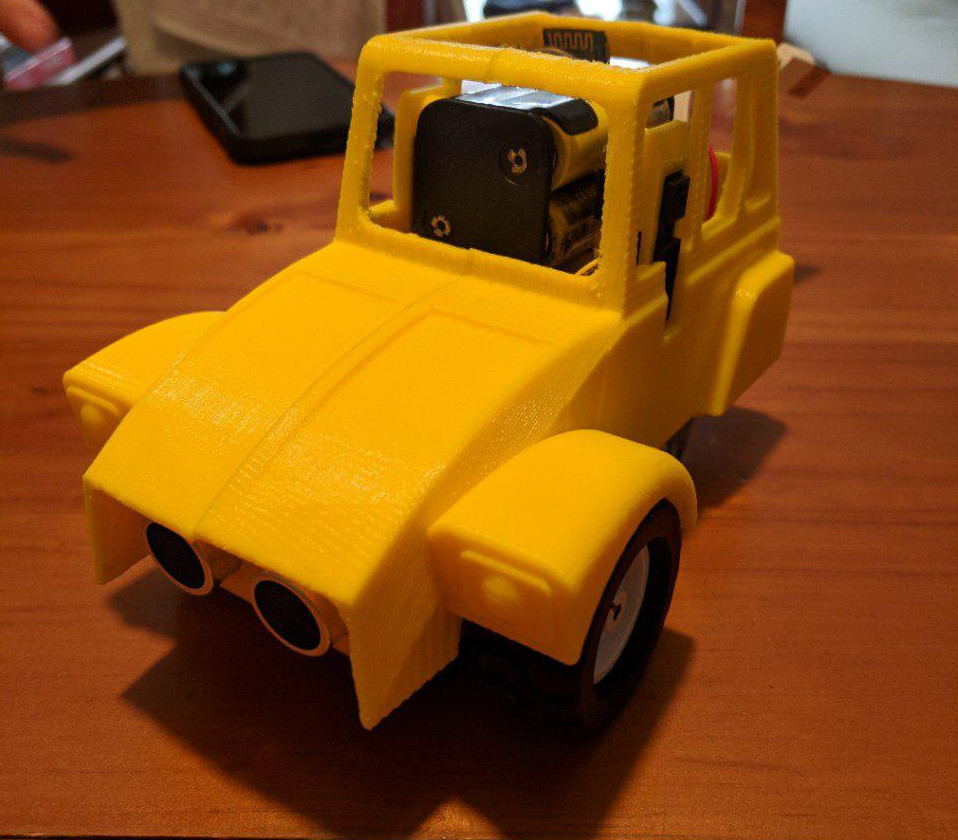
\includegraphics[width=150px, height=150px]{img/Caprito7.jpg}
  &
  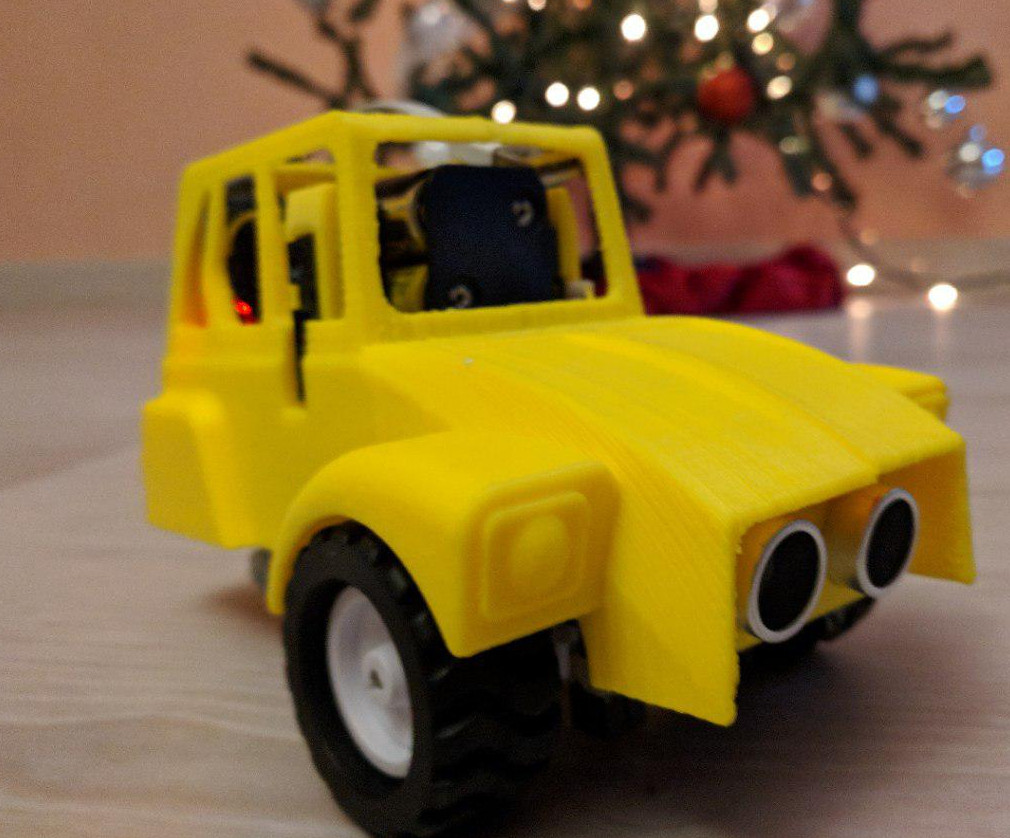
\includegraphics[width=150px, height=150px]{img/Caprito8.jpg}\\

\end{tabular}
\caption{Galería del robot}
\end{figure}

\newpage
Finalmente se incluyen algunas capturas de la aplicación móvil desarrollada:

\begin{figure}[h!]
\centering
\begin{tabular}{ccc}
  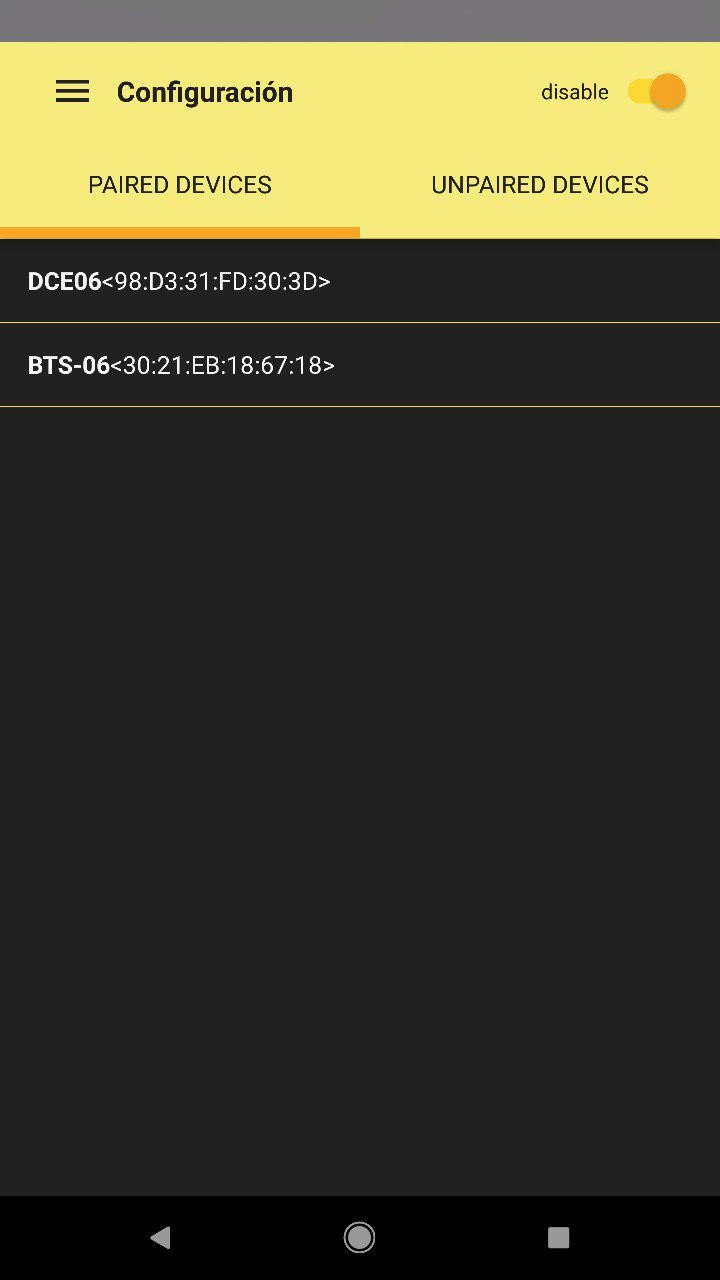
\includegraphics[scale=0.20]{img/App1.jpg}
&
  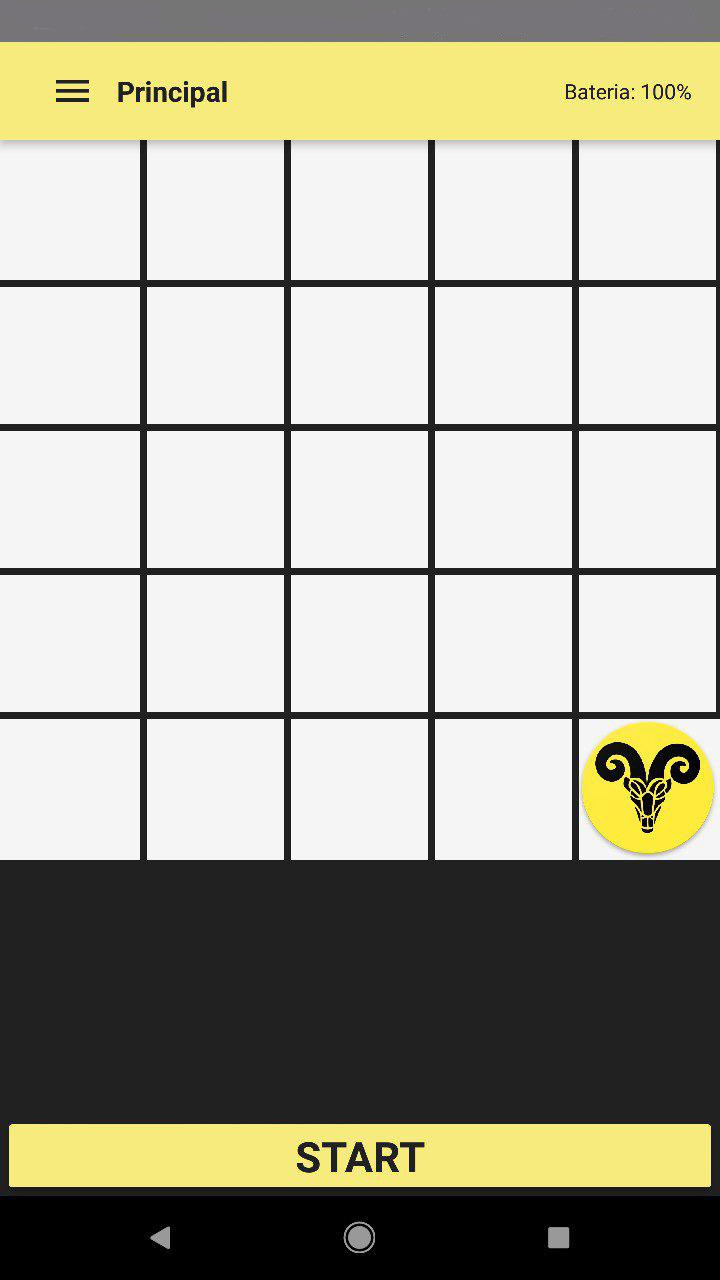
\includegraphics[scale=0.20]{img/App2.jpg}
&
  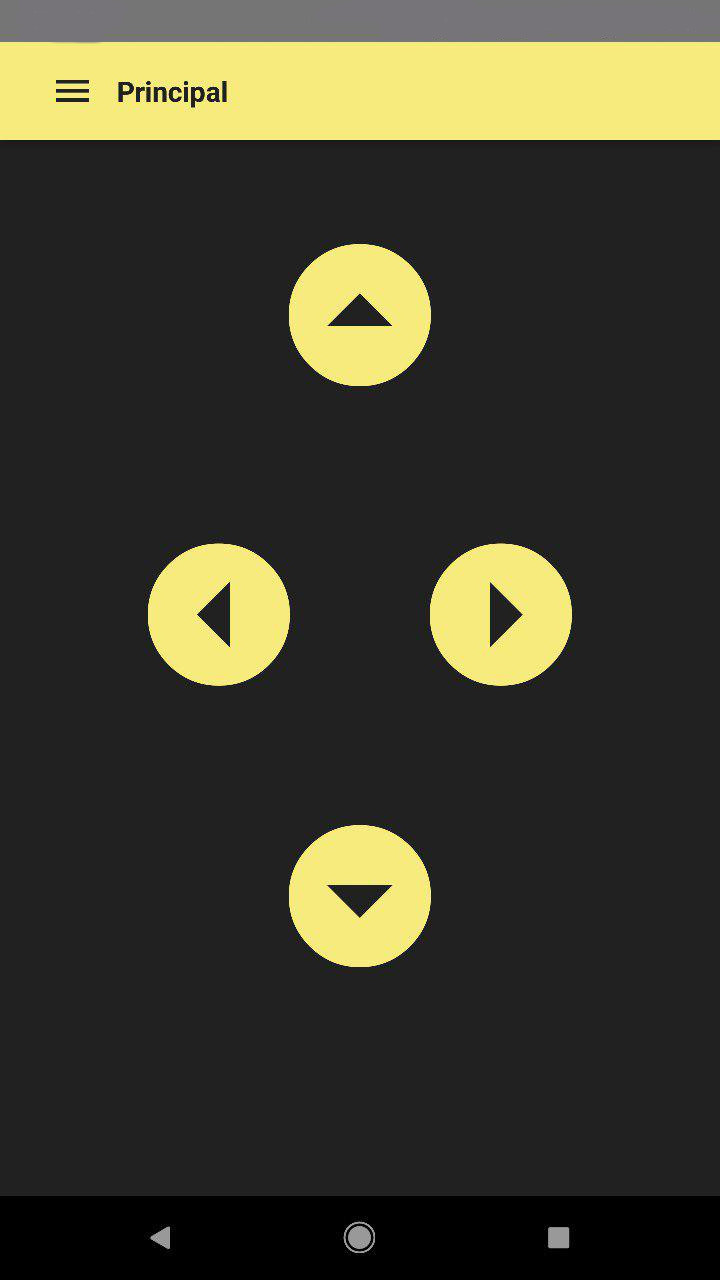
\includegraphics[scale=0.20]{img/App3.jpg}\\
\end{tabular}
\caption{Muestra de la aplicación móvil}
\end{figure}
